\documentclass{LMCS}

\def\doi{8(3:23)2012}
\lmcsheading {\doi}
{1--20}
{}
{}
{Dec.~15, 2010}
{Sep.~26, 2012}
{}
 


\usepackage[utf8]{inputenc}

\usepackage{enumerate}
\usepackage{hyperref}
\usepackage{xspace}
\usepackage{amsmath, amssymb, latexsym, amsfonts}
\usepackage{tikz}
\usetikzlibrary{automata,arrows,calc,decorations.markings}
\def\tikzscalefactor{0.7}
\usepackage{macros}
\usepackage{mathtools}
\usepackage{ifthen}


\newenvironment{definition}{\begin{defi}}{\end{defi}}
\newenvironment{theorem}{\begin{thm}}{\end{thm}}
\newenvironment{lemma}{\begin{lem}}{\end{lem}}
\newenvironment{proposition}{\begin{prop}}{\end{prop}}
\newenvironment{remark}{\begin{rem}}{\end{rem}}
\newenvironment{corollary}{\begin{cor}}{\end{cor}}

\newenvironment{claim}{\medskip\noindent\textit{Claim.\ }}{\medskip}





\begin{document}

\title[Reachability Analysis of Communicating Pushdown Systems]{Reachability Analysis of Communicating Pushdown Systems\rsuper*}

\author[A.~Heußner]{Alexander Heußner}	\address{LaBRI, Universit{\'e} de Bordeaux, CNRS -- France}	\email{\{alexander.heussner, jerome.leroux, anca, gregoire.sutre\}@labri.fr}  

\author[J.~Leroux]{Jérôme Leroux}	

\author[A.~Muscholl]{Anca Muscholl}	

\author[G.~Sutre]{Grégoire Sutre}	





\keywords{Reachability analysis, communicating processes, pushdown systems.}
\subjclass{D.2.4, F.2}
\titlecomment{{\lsuper*}An extended abstract of this paper appeared in FoSSaCS'10.}







\begin{abstract}
  \noindent The reachability analysis of recursive programs that
  communicate asynchro\-nously over reliable \fifo channels calls for
  restrictions to ensure decidability. Our first result characterizes
  communication topologies with a decidable reachability problem
  restricted to eager runs (i.e., runs where messages are either received
  immediately after being sent, or never received). 
 The problem is
  \dexptime-complete in the decidable case.  The second result is a
  doubly exponential time algorithm for bounded context analysis in
  this setting, together with a matching lower bound. Both results
  extend and improve previous work from~\cite{latorre-s-2008-299-a}.
\end{abstract}
 
\maketitle


\section*{Introduction}

Checking safety properties for distributed programs like client/server
environments, peer-to-peer applications, or asynchronous programs on
multi-core processors is a standard task in
verification. However, it is well established that the automatic
analysis of distributed programs is a quite challenging
objective. 

A basic feature of the programs used in the applications mentioned above
is that they need to exchange information asynchronously, over
point-to-point channels that are unbounded and reliable. Such
information is used for instance to perform function calls on remote
processes. This amounts to considering a model that combines recursion with
asynchronous communication. Such a combined model is similar in spirit
to, e.g., process rewrite systems~\cite{mayr}, that mix
recursion and Petri nets. We denote the combination of
recursion and asynchronous communication as~\emph{Recursive
  Communicating ProcesseS} (\rqcp for short) here. The model has been
recently studied by La\,Torre, Madhusudan, and
Parlato~\cite{latorre-s-2008-299-a}, who were mainly interested in
applying bounded context analysis to this setting.

Since \rqcp subsume the well-studied class of communicating
finite-state machines~\cite{brand-d-1983-323-a}, reachability is
already undecidable without recursion. Moreover, it is well-known that
reachability for pushdown systems that synchronize by rendezvous
 is undecidable as well~\cite{ramalingam-g-2000-416-a}.
Therefore, our main motivation was to separate these two
sources of undecidability. We consider here behavioral restrictions
for which reachability for communicating \emph{finite-state} machines
is decidable, and then look under which conditions
recursion can be added to the model.

The reachability question for communicating finite-state machines can
be tackled in three different ways, either by restricting
the communication topology, or by assuming that channels are lossy, or by
considering only executions on channels of fixed size. In general,
the last two approaches provide approximated solutions to the
reachability problem. On the positive side, the last idea yields exact
solutions in some special cases, either for certain restricted
topologies (e.g., acyclic ones) or
under certain behavioral restrictions on the communication (e.g., mutex
communication, see below).

As already mentioned, our starting point is the work of La\,Torre et
al.~\cite{latorre-s-2008-299-a}. They introduced a syntactic
restriction on the combined use of channels and pushdowns, that prevents
the synchronization of pushdowns leading to an
undecidable reachability question. An \rqcp is called \emph{well-queueing}
in~\cite{latorre-s-2008-299-a} if pushdown processes can only read
messages when their stack is empty (they can send messages without
any restriction). Well-queueing expresses an event-based programming
paradigm: tasks are executed by threads without interrupt, i.e., a
thread accepts the next task only after it finished the current
one. One of the results of \cite{latorre-s-2008-299-a} is that
well-queueing \rqcp have a decidable reachability problem if and only
if the topology is a directed forest; in the decidable case, they
provide a doubly exponential algorithm by a reduction to bounded-phase
multi-stack pushdown systems~\cite{latorre-s-2007-161-a}.

We extend the results
of~\cite{latorre-s-2008-299-a} in several directions. First, we add a
dual notion to well-queueing: a pushdown process can send messages
only with empty stack (but can read messages without
restriction). This dual notion arises naturally if one wants to model
interrupts: a server might need to accept tasks from high priority
clients independently of the status of the running task. We use these two
restrictions  by fixing the type of each communication channel, to be either
well-queueing or the dual notion. A communication topology, together
with channel types, is called a \emph{typed topology}.


We give in Section~\ref{sect:converge} a precise characterization of those
typed topologies for which the \rqcp model has a
decidable reachability problem over so-called
\emph{eager} runs. A run is eager if the
sending of a message is immediately followed by its
reception (if any). This notion is closely related to 
bounded communication~\cite{lohrey-m-2004-160-a}. 
Communicating finite-state machines with existential channel bounds,
i.e., where each run \emph{can} be
reordered into a run over bounded channels, are a
well-studied model enjoying good expressiveness and
decidability properties~\cite{genest-b-2006-920-a}\footnote{Machines with the
property that  each run can be reordered into an eager
one, are a special instance of existentially 1-bounded
machines. Eagerness is related 
to a \emph{global} channel bound~\cite{lohrey-m-2004-160-a}.}.
Here, we
simply use  eager runs in order to rule out undecidability
due to unbounded channels, since reachability for finite-state
communicating machines over eager runs is decidable. We show that reachability
of \rqcp over eager runs is \dexptime-complete in the
decidable case. Our result generalizes and improves the
doubly exponential time decision procedure of
\cite{latorre-s-2008-299-a}, which holds for topologies without undirected
cycles (called \emph{polyforests}).



The restriction to eager runs appears to be strong at a first glance.
However, we show in Section~\ref{sect:mutex} that it arises rather
naturally, by imposing a behavioral restriction on the communication:
the \emph{mutex} restriction requires that in every reachable
configuration there is no more than one non-empty channel per cycle of
the network. In particular, \rqcp over polyforest architectures are
mutex. Mutex can also be  seen as a generalization of the half-duplex
restriction studied in \cite{cece-g-1997-304-a}.


La\,Torre et al.~propose in~\cite{latorre-s-2008-299-a}  a second
approach to solve the reachability problem for \rqcp, inspired by successful
work on reachability with bounded contexts in the
verification of concurrent Boolean programs~\cite{qadeer-s-2005-93-a}.
They show that bounded-context reachability for
well-queueing \rqcp is decidable in time doubly exponential in the
number of contexts. Again, this result is obtained by a reduction to
bounded-phase multi-stack pushdown
systems~\cite{latorre-s-2007-161-a}. Our result in Section~\ref{sect:bounded}
extends the bounded-context result of~\cite{latorre-s-2007-161-a} to
\rqcp that allow for the two dual notions of well-queueing.
Moreover, our algorithm is direct and simpler than the one
involving bounded-phase multi-stack pushdown
systems. We also provide a matching lower bound for the complexity.






\medskip
\noindent{\it Related work.\ }
In the context of multi-thread programming, other notions of
synchronization between pushdowns arise naturally. Earlier
publications considered synchronization via shared memory, such as
local/global memory in
\cite{bouajjani-a-2005-348-a,bouajjani-a-2005-437-a} or bags in
\cite{sen-k-2006-300-a,jhala-r-2007-339-a}. The paper
\cite{bouajjani-a-2005-348-a} showed that bounded-context reachability
can be solved in exponential time, whereas \cite{sen-k-2006-300-a}
provided an exponential space lower bound for reachability with atomic
methods (without
context bounds).  Also, synchronization in the form of state
observation was considered in~\cite{atig-m-2008-356-a}. The latter
model was shown to be decidable only for acyclic architectures, and is
strongly related to lossy
systems~\cite{abdulla-p-1996-91-a,finkel-a-2001-63-a}.  For the shared
memory model, \cite{kidd10} shows how to reduce concurrent pushdowns
to a single pushdown, assuming a priority preemptive scheduling policy.  Lately,
\cite{seth-a-2010-615-a,atig-m-2010-117-b} proposed a general strategy
to reduce bounded-phase reachability questions on different
multi-stack pushdown automata models to a single stack. This is close
in spirit to our proof technique in Section~\ref{sect:converge},
although we do not rely on a phase-bounded model for our first
result. 










 
\section{Recursive Communicating Processes}




Given a set  and a -indexed family of sets , we 
write elements of the Cartesian product  in bold face.  For
any  in  and any , we let 
denote the -component of  .  Moreover, we identify 
with the indexed family of elements .

An \emph{alphabet} is any finite set of \emph{letters}.  Given an
alphabet , we write  for the set of all \emph{finite words}
(\emph{words} for short) over , and we let  denote the
\emph{empty word}.  


A \emph{labeled transition system} (LTS for short)
 is given by a set
of~\emph{states} , an initial state , an 
\emph{action} alphabet , and a (labeled)~\emph{transition relation}
, which is a subset of . For
simplicity, we usually write  in place of . The \emph{size} of  is defined by

when  is finite.


Throughout the paper we use standard complexity classes such as
polynomial space (\pspace), deterministic exponential time (\dexptime), and
deterministic doubly-exponential time (\twodexptime).  For detailed definitions
the reader is referred to, e.g., \cite{papadimitriou-c-1994--a}.





\subsection{Communication Topologies}

In this paper, we consider processes from a finite set , that
communicate over point-to-point, error-free \fifo channels from a set
. They exchange messages over a given  topology, which
is simply a directed graph whose vertices are processes and whose
edges represent channels:

\begin{definition}
  A \emph{topology}   is a tuple  where 
  is a finite set of \emph{processes}, and  is a finite set
  of point-to-point \emph{channels} equipped with two functions
   that map every channel  to a
  \emph{source}  and a \emph{destination}
  , such that .
\end{definition}

The \emph{size} of  is defined by .
For each channel , we write  for the binary
relation on the set of processes  defined by 
if  and . We also use the undirected
binary relation , defined by  if
 or .



An \emph{undirected path} in  is an alternating sequence
, of processes  and
channels ,
such that  for all .
Moreover, the undirected path is called \emph{simple} if the processes
 are distinct.
A \emph{simple undirected cycle} in  is an undirected path
 with 
such that  are distinct, and
 are distinct. 
The topology  is called \emph{polyforest} if it contains no
simple undirected cycle.


\subsection{Communicating  Processes}

Consider a topology .
Given a message alphabet , we denote by  the set
of \emph{possible communication actions} of a process ,
defined by .  As usual, 
denotes sending message  into channel , whereas 
denotes receiving message  from channel .
Note that  and  are disjoint when
 and  are distinct processes.



\begin{definition}
  A \emph{system of communicating processes (\qcp for short)}
   is given by a topology
  , a \emph{message} alphabet , and, for each process
  , an LTS 
  such that:
  \begin{iteMize}{}
  \item the action alphabets , , are pairwise disjoint, and
  \item  is contained in
     for each .
  \end{iteMize}
\end{definition}



\noindent Actions in  are called \emph{communication actions} of
, whereas  is the set of
\emph{local actions}. States  are called
\emph{local states} of . We write  for the
set of \emph{global states}. Note that the sets , and
hence , may be infinite.  Indeed, the local transition
systems  could be, for example, counter
or pushdown systems.  When 
is finite,  is called a \emph{finite} \qcp,
and its \emph{size} is defined by
.

\smallskip

As usual, the semantics of \qcp is defined in terms of a global LTS
, where  is the set of \emph{configurations},  is the initial configuration,
   is the set of actions, and
   is
  the transition relation with , where , if 
  the following conditions are satisfied:
  \begin{enumerate}[(i)]
  \item  and  for all  with ,
  \item if  then ,
  \item if  then  and  for all  with ,
  \item if  then  and  for all  with .
  \end{enumerate}
Given a process , we call~\emph{move} of  any transition
 with . A move is local if .

\medskip

A \emph{run} in the LTS  is a
finite, alternating sequence  of
configurations  and actions  satisfying
 for all . We say
that  is a run from  to . The
\emph{length} of  is , and is denoted by .
A run of length zero consists of a single configuration.
The \emph{trace} of a run
     is the sequence of actions
    .
A pair of send/receive
actions  is called~\emph{matching} in
 if  and the number of receives on  within
 equals the length of  in .
If  are two runs such that the last configuration of 
is equal to the first configuration of , then we write
 for their concatenation.

We
define the \emph{order-equivalence} relation  over runs as the
finest congruence such that  whenever   are actions on different processes.
Informally,  if they can be
transformed one into the other by iteratively commuting adjacent
transitions that (i) are \emph{not} located on the same
process, and (ii) do \emph{not} form a matching send/receive pair.
The following is easy to check:

\begin{fact}
  If  are order-equivalent runs of a \qcp, then
  they start in the same configuration and end in the same configuration.
\end{fact}

\medskip

A configuration  is \emph{reachable} in a \qcp  if there
exists a run of  from the initial configuration  to
.  We define the \emph{reachability set} of  as
.

\smallskip

The~\emph{state reachability problem} for \qcp asks, for a given \qcp
 and a global state , whether 
 intersects
.  It is well-known that this problem is
undecidable for finite \qcp, even if we restrict the
topology to two
processes connected by two channels~\cite{brand-d-1983-323-a}.













The undecidability of the state reachability problem for \qcp is based on
the fact that one cannot control how ``fast'' messages are received.
A simple idea that rules out such behaviors is to consider only runs
where the reception is immediate (if it exists):

\begin{definition}
  A run  is \emph{eager} if for all
  , if  is a receive action then  and
   is its matching send action. \label{def:bounded_run}
\end{definition}
Thus, each send action along an eager run is either immediately
followed by its matching receive, or it is never matched.  In
the latter case, all later sends into the channel are never received,
and we say that the channel is in its ``growing phase''.  In the
former case, the adjacent matched send/receive actions act like a
rendezvous synchronization between the two processes.  Formally, given
a channel , we call \emph{rendezvous on } any run (of
length~2)  such that  with . The rendezvous~\emph{involves
  process } if .


We introduce now the ``eager'' variants of the reachability notions
presented previously.  A configuration  is
\emph{eager-reachable} in a \qcp  if there exists an eager run
from the initial configuration  to .  The
\emph{eager-reachability set} of  is the set
 of eager-reachable configurations.  We say that
a \qcp  is~\emph{eager} when . In the next section, we show how eager \qcp 
occur under some natural (and decidable) restrictions on cyclic
communication. The simplest example arises over polyforest
topologies. 



The \emph{state eager-reachability problem} for \qcp
asks, for a \qcp  and a global state , whether  intersects .  It is readily seen that this problem is decidable for
\emph{finite} \qcp in \pspace.

Eager runs, modulo the fact that Definition~\ref{def:bounded_run}
allows for runs which end in a sequence of (unmatched) send actions,
are closely related to the notion of globally 1-bounded runs. Eager
\qcp subsume existentially globally 1-bounded communicating
machines~\cite{lohrey-m-2004-160-a,genest-b-2007-1-a}. However, as we
will see in Section~\ref{sect:mutex}, it is undecidable whether a
finite \qcp is eager (in contrast, one can decide whether a finite,
deadlock-free communicating machine is existentially globally 1-bounded~\cite{genest-b-2007-1-a}). On the
positive side, Section~\ref{sect:mutex} shows a decidable subclass of
finite, eager \qcp.







 \subsection{Recursive Communicating Processes}\label{ssec:rqcp}

In the following we introduce \rqcp together with a symmetric version
of the ``well-queueing'' restriction used in
\cite{latorre-s-2008-299-a}.
Informally, \rqcp (recursive \qcp) are  \qcp where each local
transition system is a pushdown system.


A well-queueing \rqcp in
\cite{latorre-s-2008-299-a} is one where a process can only receive
when its stack is empty. Here, we dualize this concept by also allowing
channels where the sender (but not the receiver) must have an empty
stack. Well-queueing was motivated
in~\cite{latorre-s-2008-299-a} by the case where recursive processes
need to finish their tasks before accepting new ones. Adding the dual notion
of well-queueing is interesting when modeling interrupts: a
recursive process may have to interrupt its current task to treat one
with a higher priority, hence, it has to preserve its current state on
the stack to return later.

\begin{definition}
  A \emph{typed} topology  consists of a topology
  , together with a \emph{type} , such that  implies .
\label{def:oriented}
\end{definition}

Given a process  and a channel , we call
~\emph{restricted} on  if  (and
\emph{unrestricted} otherwise). Informally, a communicating pushdown
process  as defined below will be restricted on  if 's stack
must be empty when communicating over channel .
































\begin{definition} 
  A \emph{pushdown system}  is given by a finite set  of
  \emph{control states}, an \emph{initial control state} , an alphabet  of \emph{actions},
  a subset ,
  a stack alphabet , and
  a transition relation , such that
   contains the set 
  of \emph{stack actions}.
\end{definition}
We define the \emph{size} of  by .
Actions in  are tests for
empty stack.
Naturally, for a pushdown system embedded in a \qcp, the set of actions
 may contain communication (and local) actions.
Depending on the typed topology, some communication actions
may require an empty stack.  This will be enforced by putting these
communication actions in the set .

According to the informal description given above, we define now the
semantics of pushdown processes.
The semantics of 
is the LTS  with set of states
, initial state ,
and (labeled) transition relation  defined as expected:
stack actions  and  behave as usual ( blocks
if the top of the stack is not ), actions from 
do not change the stack, and actions in  are possible only if
the stack is empty.



\begin{definition}
  A \emph{recursive \qcp} (\rqcp for short)
   is given by a typed
  topology , a~\emph{message} alphabet , and,
  for each  process ,  a
  pushdown system
   such that:
  \begin{iteMize}{}
  \item the action alphabets , for , are pairwise disjoint,
  \item  is contained in
     for each , and
  \item  for each .
  \end{iteMize}
\end{definition}
We associate with  the \qcp 
where, for each , the LTS  is the semantics of the
pushdown system .
The \emph{size} of  is defined by
.



\smallskip

We write  for the set
\emph{global control states}.
Abusing notation, a global state  of  will also be written
 where  for each .
The~\emph{state reachability problem} for \rqcp
asks, for a given \rqcp
 and a global control state , whether

intersects
.
The \emph{state eager-reachability problem} for \rqcp is defined similarly,
using  instead of .


 \section{Topologies with Decidable State Reachability}
   \label{sect:converge}

   Several factors lead to the undecidability of the state
   reachability problem for \rqcp.  In particular, the model is
   already undecidable without any pushdown.  Our goal in this section
   is a decidability condition that concerns the interplay between
   pushdowns and communication, assuming that the communication is
   \emph{not} the reason for undecidability.  For this reason, we consider a
   restricted version of the state reachability problem, namely the
   one on eager runs. 


\begin{definition}\label{def:conv}
  A typed topology  is called
  \emphconverging if it contains a simple undirected path
  , with , such that
   is unrestricted on  and  is unrestricted on .
\end{definition}

Notice that non-\convergence
implies that
every channel is either restricted
at the source, or at the destination, or at both ends
(see Figure~\ref{fig:non-confluent-examples}).

\begin{figure}[b]
  \centering
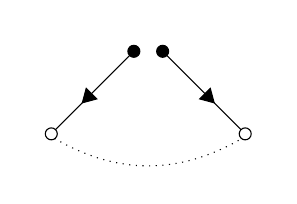
\begin{tikzpicture}[
  node distance=2cm,
  decoration={
    markings,
    mark=at position 0.62 with {\arrow{triangle 60}}
  }]

  \node (p)  {};
  \node (q1)  [below left of=p]  {};
  \node (qn)  [below right of=p] {};

  \draw      (p) edge [*-o] (q1)
  [decorate] (p) to         (q1)
  ;
  \draw      (p) edge [*-o] (qn)
  [decorate] (p) to         (qn)
  ;

  \draw [dotted, bend angle=30, bend right]
  ([xshift=1mm] q1.north east) to ([xshift=-1mm] qn.north west)
  ;
\end{tikzpicture}
\hspace{0.75cm}
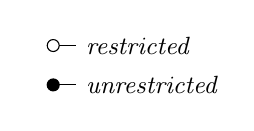
\begin{tikzpicture}[node distance=0.5cm]
  \node (p)  {};
  \node (p') [right of=p, anchor=west]  {\small\em restricted};
  \node (q)  [below of=p] {};
  \node (q') [right of=q, anchor=west] {\small\em unrestricted};

  \draw (p) edge [o-] (p')
        (q) edge [*-] (q')
  ;
\end{tikzpicture}
 \hspace{0.75cm}
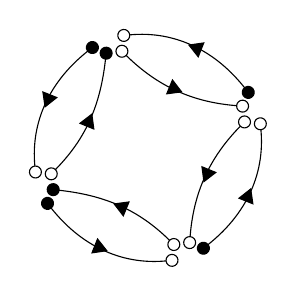
\begin{tikzpicture}[
  proc/.style = {}
  ]

   \draw (20:1.5)  node[proc] (1) {};
   \draw (110:1.5) node[proc] (2) {};
   \draw (200:1.5) node[proc] (3) {};
   \draw (290:1.5) node[proc] (4) {};

   \begin{scope}[
     decoration={
       markings,
       mark=at position 0.54 with {\arrow{triangle 60}}
     }]

     \draw      (1) edge[*-o,bend right=30] (2)
     [decorate] (1) to  [    bend right=30] (2)
     ;
     \draw      (2) edge[*-o,bend right=30] (3)
     [decorate] (2) to  [    bend right=30] (3)
     ;
     \draw      (3) edge[*-o,bend right=30] (4)
     [decorate] (3) to  [    bend right=30] (4)
     ;
     \draw      (4) edge[*-o,bend right=30] (1)
     [decorate] (4) to  [    bend right=30] (1)
     ;
   \end{scope}

   \begin{scope}[
     decoration={
       markings,
       mark=at position 0.46 with {\arrowreversed{triangle 60}}
     }]

     \draw      (1) edge[o-o,bend left=20] (2)
     [decorate] (1) to  [    bend left=20] (2)
     ;
     \draw      (2) edge[*-o,bend left=20] (3)
     [decorate] (2) to  [    bend left=20] (3)
     ;
     \draw      (3) edge[*-o,bend left=20] (4)
     [decorate] (3) to  [    bend left=20] (4)
     ;
     \draw      (4) edge[o-o,bend left=20] (1)
     [decorate] (4) to  [    bend left=20] (1)
   ;
   \end{scope}
\end{tikzpicture}
  \caption{Examples of non-\converging typed topologies}
  \label{fig:non-confluent-examples}
\end{figure}

We say that a typed topology  has a decidable \rqcp state
eager-reachability problem if the latter question is decidable for the class of
\rqcp with typed topology .  We show in this section that the notion of
\convergence gives a complete characterization of typed topologies
with respect to the decidability of the above problem.

\begin{theorem}\label{thm:conv}
  A typed topology has a decidable \rqcp state
 eager-reachability problem  if and only if it is non-\converging.
  Moreover, the problem is \dexptime-complete in the latter case.
\end{theorem}

The rest of the section is devoted to the proof of this theorem.
We first show the undecidability result in the \converging case.

\begin{proposition}
  Every \converging typed topology has an undecidable \rqcp
  state (eager-) reachability problem. 
\end{proposition}
\begin{proof}
  Consider a typed topology  that is \converging.  There
  is a simple undirected path 
  satisfying the conditions of Definition~\ref{def:conv}.
  Since  is unrestricted on  and  is
  unrestricted on , both may use their stack while communicating
  over the channels  and , respectively. 
  Recall that checking non-emptiness of the intersection of two context-free languages is undecidable.
  To prove the lemma, we reduce this problem to the state
  eager-reachability problem for \rqcp with typed topology .

  Given two context-free languages  and  over the alphabet
  , the process  guesses a word in
   while  guesses a word in , and both processes check that
  they guessed the same word via synchronizations along the undirected path . 
  Intermediate processes  do not use their
  stack, they simply convey the information about the common input
  guessed by  and .  The labeled transition system
  , , is depicted below.


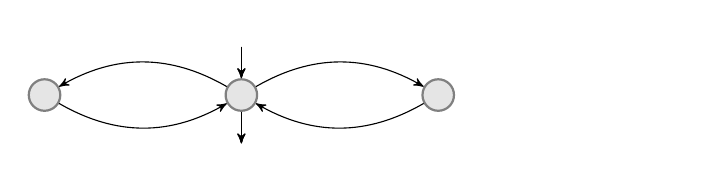
\begin{tikzpicture}[node distance=2.5cm, >=stealth', bend angle=30]
  \tikzstyle{initial}   = [initial   by arrow, initial   text=, initial   above, initial   distance=0.4cm]
  \tikzstyle{accepting} = [accepting by arrow, accepting text=, accepting below, accepting distance=0.4cm]

  \tikzstyle{every state} = [draw=gray, thick, fill=gray!20, minimum size=4mm, inner sep=2pt]

  \node [state]  (q1)  [initial, accepting]         {};
  \node [state]  (q2)  [left of=q1]      {};
  \node [state]  (q3)  [right of=q1]     {};
  \node                [right of=q3, node distance=3cm]     {};

  \path[->]  (q1)  edge [bend right]  node [above]   {}     (q2)
             (q2)  edge [bend right]  node [below]   {}     (q1)
             (q1)  edge [bend left]   node [above]   {} (q3)
             (q3)  edge [bend left]   node [below]   {} (q1)
  ;
\end{tikzpicture}

  Similarly, the pushdown systems  and  are obtained
  from pushdown automata accepting  and , respectively, by replacing
  tape-reading actions with communications (
  for  and  for ).

 Finally, we only need to make sure that the channels are empty at the end.
  As usual, this can be enforced by augmenting  with a new symbol
  }\mathtt{\ on each
  channel  at the end of the simulation. 

The construction guarantees that the intersection  is
non-empty if and only if there is an (eager) run in the \rqcp from the
initial configuration to a global control state where each process is
accepting. 
\end{proof}



We now focus on non-\converging typed topologies.
Let us first prove the \dexptime lower bound of
Theorem~\ref{thm:conv}.

\begin{proposition} \label{prop:non-confluent-lb} The state
 eager-reachability problem for  \rqcp
  with non-\converging typed topology is  \dexptime-hard.
\end{proposition}

\begin{proof}
It is well-known (and probably folklore) that the following problem is
\dexptime-complete: 
given a context-free language  and  regular languages ,
check the non-emptiness of .
The hardness follows easily by a reduction from linearly bounded
alternating Turing 
machines.
Actually, a closely related problem is shown to be \dexptime-hard
in~\cite{esparza-j-2003-355-a}, namely the reachability problem for
pushdown systems with
checkpoints.

Notice that the intersection  can be simulated
on the non-\converging, 
typed topology  where
, , and,
for each ,
 with  unrestricted on  and
 restricted on  (see left part of
Figure~\ref{fig:non-confluent-examples}). That is, process 
simulates a pushdown automaton accepting the context-free language
, whereas process  simulates a finite-state automaton
accepting . Communication guarantees that the simulations
use the same input word. As in the previous proposition, one needs to
enforce the emptiness of the channels by using an extra symbol.
\end{proof}


Before considering the upper bound we need to introduce some
vocabulary. Consider a run  of an
\rqcp .  Given a process , we say that  is
\emph{well-formed for } if the projection of  on  is a  Dyck word.  This
well-formedness condition merely stipulates that each push action of
 in  is matched by a pop action, and vice versa.  We
call  \emph{well-formed} if  is well-formed for each
process .  For instance, every run that starts and ends with
empty stacks  is well-formed.  A stronger condition is that of
well-bracketing, which requires that push and pop actions for distinct
processes must be nested recursively.
Formally, we say that  is
\emph{well-bracketed} if the following two conditions are satisfied:
\begin{enumerate}
\item
  the projection of  on the disjoint union
   is a Dyck word, and
\item
  for every process  and every ,
  if the pairs  and  are matching push/pop actions
  of , then the sub-runs  and
   are
  well-formed for all .
\end{enumerate}
Observe that if  is defined, then  is
well-formed (resp.~well-bracketed) if   and  are both
well-formed (resp.~well-bracketed).  Note also that well-formedness is
preserved under order-equivalence: if  is well-formed and  then  is also well-formed.  However,
well-bracketing is not preserved under order-equivalence.


The following proposition provides the main ingredient to show the
 upper bound of Theorem~\ref{thm:conv}.

\begin{proposition} \label{prop:wf-to-wb-for-confluent} Given an \rqcp
   with non-\converging typed topology, every eager,
  well-formed run in  is
  order-equivalent to an eager, well-bracketed run. 
\end{proposition}

\begin{proof}
  By induction on the length of runs.
  The basis is trivial.
  Consider a run , of non-zero length, that is both eager and well-formed.
  We assume that  starts with a push action (otherwise, the existence of an order-equivalent run that is both eager and well-bracketed immediately follows by induction).
  Let  denote the first action of , and let  denote the process with .
Let  denote an order-equivalent eager run obtained from  by scheduling the actions of  as early as possible, while maintaining adjacent send/receive pairs.
  It is readily seen that  may be written as:

  where the runs ,  and  satisfy the
  following conditions:
  \begin{enumerate}[(a)]
  \item\label{enum:decomp-only-p}
     consists of moves of process  which are either
    local actions or
    sends that are unmatched in ,
  \item\label{enum:decomp-only-not-p}
    contains no move of process ,
  \item\label{enum:decomp-sync}
    is a rendezvous involving ,
  \item\label{enum:decomp-wf}
the transitions  and  are matching stack actions (of
  process ), 
  \item\label{enum:schedule-p-first}
    for each , the run  is not
    order-equivalent to a run of the form  where  and  is a
    rendezvous involving .
\end{enumerate}
The scheduling of 's actions as early as possible is expressed by
  condition~(\ref{enum:schedule-p-first}) (notice that  and
   correspond to the same send/receive pair). 
  
  \noindent
  We first show the following claim.

  \begin{claim}
    For each , all processes that move in 
    have an empty stack at the start and end of . 
  \end{claim}

  To prove the claim, let us denote by 
  the set of processes that move in , ordered by their last
  occurrence in . 
  Since the last action in  is performed by , 
  we derive from~(\ref{enum:schedule-p-first}) that the rendezvous
   is on a channel between  and . 
  Now let .  It follows
  from~(\ref{enum:schedule-p-first}) that the last action of  in
   is a communication action .  We have two cases to
  consider: 
  \begin{iteMize}{}
  \item  is a send action: If there was no matching receive in , then this send action could be scheduled after , contradicting~(\ref{enum:schedule-p-first}).
    Hence,  contains a matching receive, which, by eagerness, is the next action in .
    This matching receive is performed by a process  with .
  \item  is a receive action: Since  is eager, the matching send is the previous action in .
    This matching send is performed by a process .
    Moreover, we must have  since, otherwise, this matched send/receive pair could be scheduled after , contradicting~(\ref{enum:schedule-p-first}).
  \end{iteMize}
  We obtain that, for every , the last action of 
  in  is a communication action over a channel 
  satisfying  for some .
  Let  denote the channel of the rendezvous , and recall that .
  Observe that  is unrestricted on  since, according to~(\ref{enum:decomp-wf}), the stack of  is non-empty in .
  As the typed topology of  is non-\converging, we derive that
   is restricted on  for each , since there
  is a simple undirected path  for each . 
It follows that  has an empty stack at the end of .


  We have thus shown that, for each , all processes
  that move in  have an empty stack at the end of .
  Now, recall that  is well-formed since it is order-equivalent
  to .  Therefore, all processes that move in  also have
  an empty stack at the start of , which concludes the proof
  of the claim.


  It follows from the claim that each run  is well-formed, so
   is also well-formed.  Since the runs
   and  are eager, we derive from the induction
  hypothesis that each  is order-equivalent to a run 
  that is both eager and well-bracketed, and, similarly,  is
  order-equivalent to a run  that is both eager and
  well-bracketed.  Replacing in  each  by  and
   by ,  yields a run  that is both eager and well-bracketed (the second condition
  for well-bracketed runs is satisfied since the runs  contain
  no move of ).  This concludes the
  proof of the proposition.
\end{proof}



Well-bracketed runs in an (arbitrary) \rqcp cannot exploit the full
power of the multiple stacks.  Indeed, the well-bracketing property
ensures that the individual process stacks do not ``interact'' with
each other: a single, global stack is sufficient to simulate the run.
More precisely, given an \rqcp , with
 for each , we
construct a product pushdown system  that simulates the
well-bracketed eager runs of .  Its set of control states is
.  A control state  means
that  is the active process,  is the current global
control state,  is the set of processes that have an empty 
stack, and  is the set of channels that are ``growing'', i.e., for
which no receive action is possible anymore.  The stack alphabet of
 is the disjoint union . The
stack of  will be the concatenation of 
words , one for each process , where  is empty if
and only if .

Let us explain how the simulation of eager, well-bracketed runs works.
First, an active process  is non-deterministically chosen, leading
to the control state .
Then,  simulates the behavior of  as expected, using
its stack as  would do, but also updates the set  accordingly. 
To simulate send actions ,  non-deterministically
decides whether  is actually part of a rendezvous  on 
(provided that ), or will never be matched. 
In the former case,  simulates (in a single step) the
rendezvous .
In the latter case, the channel  is added to the set  of
``growing'' channels. 
Moreover, in both cases, the communication is performed only if the
typed topology allows it, which can be checked using the set . 

The pushdown system  may choose
non-deterministically, at any
time, to switch the active process to
some process .  
Since the run simulated by  is well-bracketed, either
's stack is empty () or 
the top stack symbol must belong to . Thus,  
performs this check and then sets  the active process to .


By construction, the pushdown system  simulates all runs
of  that are both eager and well-bracketed, and only those
runs. Moreover, the size of  is bounded by
. Since every \rqcp can be easily
modified in order to reach a given state with all stacks empty we
obtain:

\begin{proposition}\label{prop:confl-reduction}
  State eager-reachability of an \rqcp of size  with
  non-\converging typed topology  
  reduces in \dexptime to state reachability for a pushdown system of
  size .
\end{proposition}


Since the state reachability problem for pushdown systems is decidable in
deterministic polynomial time, we obtain the upper bound:

\begin{proposition}\label{prop:eager-upperb}
  The state eager-reachability problem for \rqcp over a
  non-\converging typed topology  is in \dexptime.
\end{proposition}
 \section{Eager \qcp and the Mutex Restriction}
\label{sect:mutex}

The previous section showed how to decide the state
eager-reachability problem provided that the topology behaves well
w.r.t.~pushdowns and communication. A
first natural question is whether one can decide if eager runs
suffice for solving the reachability problem. A second legitimate
question is whether the restriction to eager runs is realistic. We
answer to the first question negatively.  However, on the positive
side we show a restricted class of \qcp where eager runs suffice:
\qcp over cyclic topologies with the mutex restriction. We focus in
this section
on \qcp since the eager condition talks about communication only.

\begin{definition}
   A configuration  of a \qcp  is \emph{mutex} if for every simple
   undirected cycle  in the topology of
   , at most one of the channels  is non-empty in .
   A run  in  is \emph{mutex} if each configuration in
    is mutex.
\end{definition}
A \qcp  is called \emph{mutex} if every configuration reachable in
 is mutex.
We show later in this section that the mutex property is decidable for
finite \qcp.
Notice also that every \qcp with polyforest topology is mutex.

\smallskip

Before discussing mutex we first comment on the results
of~\cite{latorre-s-2008-299-a} and explain their relation with
Theorem~\ref{thm:conv} and Corollary~\ref{c:mutex} below.
The latter paper shows that state reachability is
decidable for finite \qcp over polyforest topologies, and for
well-queueing \rqcp over directed forests.  The proof of the result
for \rqcp relies on the idea that, on tree topologies, one can
reorder runs such that the resulting run has a bounded
number of contexts, where in each context only
one process executes all its actions by reading on one unique
incoming channel from its tree parent (and---in the case of
\rqcp---solely when its local stack is empty). Hence, the
problem reduces to the control-state reachability for a bounded-phase
multi-stack pushdown system, a question which was proven to be decidable in
doubly exponential time~\cite{latorre-s-2007-161-a}. A simple channel
reversal argument allows us to reduce the question for finite \qcp over
polyforest topologies to directed forests.

We show in the following that mutex \qcp are eager.  This
allows us to apply the results of the previous section and to obtain
the decidability of state reachability (for both finite \qcp
over polyforest topologies and well-queueing \rqcp over directed
forests)  via a direct
proof. Moreover, recall that the complexity of the algorithm of the
previous section is \dexptime, so one exponential less than the
results obtained  in~\cite{latorre-s-2007-161-a} for polyforest architectures.

\begin{remark}
  Over a topology of two finite
  processes connected by two channels, mutex runs are referred to as
  ``half-duplex communication''.
  For these, it is known how to decide the
  reachability problem through an effective construction of the
  recognizable reachability set~\cite{cece-g-2005-166-a}.
  Quasi-stable  systems are a semantic ad-hoc extension of
  this idea to finite \qcp with larger, cyclic
  topologies~\cite{cece-g-1997-304-a}.
\end{remark}



\begin{proposition}
  \label{p:one-bound}
  Given a \qcp , every mutex run starting with empty channels
  admits an order-equivalent eager run.
\end{proposition}
\begin{proof}
  By induction on the length of runs.
  The basis is trivial.
  Consider a mutex run  of non-zero length, that starts with
  empty channels. In particular, each receive action in
   has a matching send in .
  We write  for the (non-empty) set of all processes
   that move in .
  For each , let  denote the last action of  in
  .
  If some  is a local action, or a send action that is not matched in
  , we may schedule it last, which preserves the run's mutex property,
  and derive the existence of an eager run  by induction.
  Otherwise, for each , the action  is a communication
  action that is matched in , and we let  denote the channel of
  .
  Note that each , for , is a channel between  and
  another process in , which we call its last peer.
  We may build an infinite sequence of processes in  by picking an
  arbitrary process in  and iteratively moving to its last peer.
  By the pigeonhole principle, there exist  in ,
  with , such that  is
  an undirected path in  and  are distinct.
  Moreover, we may assume w.l.o.g. that  is the process that moves
  last in  among .
  To simplify notation, let us simply write  in place of ,
  and  in place of .
Remark that the undirected path  must
  be a simple undirected cycle if .

  Let us show that  is a pair of matching send/receive actions.
  Since  and  stops moving before  in
  , the communication action , which is matched in ,
  must be a receive action .
  We obtain that  is of the form:
  
  with no move of  in , and no move of  in .
  It follows that  is non-empty in .
  Since  is a mutex run,  and  are mutex configurations.
  If , then  is also non-empty in , hence 
  must be empty in both  and , which is impossible since 
  is communication action on .
  Therefore, we get that , and, hence,  is the last send
  action on  in .
  Since  is matched in , it follows that  is the matching
  send of , which implies that .

  We may now conclude the proof of the proposition.
  Recall that  are the last actions of  and  in
  , respectively.
  Since  and  are matched,
  we may schedule  last.
  This leads to a run  that is order-equivalent to , and of
  the form:
  
  where the trace
  of  satisfies
  .
  It follows from the previous trace equality that, for each configuration
   occurring in , there exists
  \begin{iteMize}{}
  \item
    either a configuration  in  with
    ,
  \item
    or a configuration  in  such that
     and  for all .
  \end{iteMize}
  In both cases, we derive that  is mutex since
   is mutex.
  Therefore, the run  is mutex.
  Moreover, the run  is also mutex since it is a prefix of the mutex
  run .
  We derive from the induction hypothesis that  is
  order-equivalent to an eager run .
  Replacing  by  in  yields a run
   that is eager.
  This concludes the proof of the proposition.
\end{proof}

\begin{corollary} \label{c:mutex}
  Every mutex \qcp is eager.
\end{corollary}

\begin{remark}
  A closer look at the proof of Proposition~\ref{p:one-bound} shows
  that the result still
  holds for the following weaker variant of the mutex property:
  a configuration  of a \qcp  is \emph{weakly mutex} if for
  every simple undirected cycle  in the
  topology of , at most one of the channels  is
  non-empty in .
\end{remark}

We derive the following result as an immediate consequence of
Corollary~\ref{c:mutex}. The upper bound is obtained as an on-the-fly
simulation: since we simulate eager runs we do not have to store any
message, but  keep track of growing
channels. The lower bound follows from
the non-emptiness test of the intersection of several regular languages.

\begin{proposition} \label{thm:mutextoeager}
  The state reachability problem for finite, mutex \qcp
  is \pspace-complete.
\end{proposition}

\begin{remark}
  State reachability remains decidable for particular
  \emph{infinite-state} mutex \qcp. For example, if each local
  LTS  is a Petri net (i.e., the \qcp in question
  is a \fifo net~\cite{finkel-a-1987-106-a}), then the state
  reachability problem reduces to the Petri net reachability
  problem, which is known to be
  decidable~\cite{mayr-e-1984-441-a,kosaraju-s-1982-267-a}.
  \label{rem:qcp_local_dec}
\end{remark}

We end this section by showing that, for finite \qcp, the mutex
property is decidable (unlike the eager one).

\begin{proposition} \label{thm:testmutex}
  The question whether a finite \qcp is mutex, is \pspace-complete.
\end{proposition}
\begin{proof}
  Assume that  is not mutex and consider a run 
  of minimal length from  to a configuration
   that is not mutex.
  By minimality, all configurations in  up to 
  are mutex.
  Let  be the predecessor of  in .

  By Proposition~\ref{p:one-bound} we can reach  by an eager
  run  (which is generated on-the-fly in \pspace) and test whether
  there exists in  a transition  that
  violates the mutex condition for .  We guess  in \pspace
  (see remark above) and check
  whether there exists a simple undirected cycle 
  in the topology of  such that one channel  is non-empty in 
  and the action  would write on another channel of this cycle
  (i.e.,  for some ).


  \pspace-hardness follows, again, by reducing from the non-emptiness
  test of the intersection of several regular languages.
\end{proof}

\begin{proposition}
  The question whether a finite \qcp is eager, is undecidable.
\end{proposition}
\begin{proof}
  We show a reduction from the universality problem for rational
  relations~\cite{berstel79}. Given such a relation
  , we ask whether .
  Here,  is described by a finite automaton  over the alphabet
  .

  We describe a finite \qcp over four processes, called ,
  and four channels  satisfying
  ,
  ,
  ,
  .
  Process  is described in Fig.~\ref{fig:P0}.
  The ingoing (outgoing, resp.) edges of  lead to the
  initial state (from the final states, resp.). Transition labels
   in  are replaced by , and labels
   are replaced by .

  Process  is described in Fig.~\ref{fig:P1}.
  The LTS  of processes  consist of a
  single (initial) state without any transition.
  Therefore, when talking about ``state components'' below we only mention
  processes .

\begin{figure}
  \centering
\begin{tikzpicture}[node distance=3cm, >=stealth', bend angle=30]
  \tikzstyle{every state} = [draw=gray, thick, fill=gray!20, minimum size=4mm, inner sep=2pt]

  \node[state,initial] (q_0)         {};
  \node[state]	(q_1) [right of=q_0] {};
  \node[state]	(q_2) [right of=q_1] {};
\node		(q_5) [rectangle,draw,below of=q_1,node distance=2cm,inner sep=5pt] {};

  \path[->] (q_0) edge              node [below]       {}\varepsilonc_{10} ? \mathtt{\}     (q_2)
                  edge [loop above, min distance=7mm, in=60, out=120] node [above]       {} (q_1)
            (q_5) edge [bend right] node [below right] {}                     (q_2);
\end{tikzpicture}
  \caption{Process  ()}
  \label{fig:P0}
\end{figure}

\begin{figure}
  \centering
\begin{tikzpicture}[node distance=3cm, >=stealth', bend angle=40]
  \tikzstyle{every state} = [draw=gray, thick, fill=gray!20, minimum size=4mm, inner sep=2pt]

  \node[state,initial] (q_0)	{};
  \node[state]	(q_1) [right of=q_0] {};
  \node[state]	(q_2) [right of=q_1] {};

  \path[->] (q_0) edge              node [above] {}\varepsilonc_{01} ? \mathtt{\} (q_2);
\end{tikzpicture}
  \caption{Process }
  \label{fig:P1}
\end{figure}

  The only runs of the above \qcp that cannot be reordered into an eager
  run are produced by  and  using all four
  }(2,5)\varepsilonc_{01}c_{10}A^*c_{02}B^*c_{03}K = A^* \times B^*\tuple{\Topo,\tau}cccccpcpcpcddcpcpcpcddpcpc\rhok\rho=\rho_1 \cdots \rho_k\rho_jx\in Xk\Rqcpk\Rqcpx_\initxk\Rqcp\Reach_k(\Rqcp)x \in Xk\Rqcp\Rqcp\vec{z} \in
\vec{Z}k\Reach_k(\Rqcp)\{\vec{z}\} \times (\prod_{p \in P}
(\Gamma^p)^*) \times (M^*)^C\phi=(p,\Pdp,z_F)p \in P\Pdp=(Z,z_I,A,A_\epsilon,\Gamma^p,\Delta)pz_F \in ZA_\actcom|\phi|\phi\Pdp\phi\xrightarrow{\phi}(\prod_{p \in P} (\Gamma^p)^*)
\times (M^*)^C(\vec{u}_I,\vec{v}_I)\xrightarrow{\phi}(\vec{u}_F,\vec{v}_F)(\vec{z}_I,\vec{u}_I,\vec{v}_I)(\vec{z}_F,\vec{u}_F,\vec{v}_F)q\not=pp\Pdp\Phi=(\phi_1,\ldots,\phi_k)\Phi=(\phi_1,\ldots,\phi_k)|\Phi|=|\phi_1|+\cdots+|\phi_k|\sqsubseteq\phi\sqsubseteq
\psi\phi\psi\phi\psi(\phi_1,\ldots,\phi_{k})\sqsubseteq
(\psi_1,\ldots,\psi_{k})\phi_j\sqsubseteq \psi_jj\Phi=(\phi_1,\ldots,\phi_k)F|F|\leq |\Phi|^k\mathcal{O}(|F|)\PhiF\Psi=(\psi_1,\ldots,\psi_k)\in F\bullet|\Psi|\leq 2|\Phi|^2\Psi\sqsubseteq \Phij\psi_j\phi_j\Phij\phi_jj\phi_j\phi=(p,\Pdp,z_F)\Pdp=(Z,z_I,A,A_\epsilon,\Gamma,\Delta)\bar{\phi}=(p,\bar{\Pdp},z_I)\bar{\Pdp}=(A,z_F,A,A_\epsilon,\bar{\Delta})\Pdp(\vec{u},\vec{v})\xrightarrow{\phi}(\vec{u}',\vec{v}')(\vec{u}',\vec{v}')\xrightarrow{\bar{\phi}}(\vec{u},\vec{v})(\phi_1,\ldots,\phi_k)(\bar{\phi}_k,\ldots,\bar{\phi}_1)\phi\bar{\phi}j\phi_j\phi_j=(p,\Pdp,z_F)\Pdp=(Z,z_I,A,A_\epsilon,\Gamma,\Delta)\phi_j\phi_jcp\Phi^\varepsilon\Phij\Phi^\pi=(\phi_1^\pi,\ldots,\phi_k^\pi)\Phi^\pi\pi=(z_r)_{s\leq r\leq j}z_r\in Zs<j\Phi^\pi\Phi^\pi\sqsubseteq \Phi\phi_j^\pi\phi_j^\pi\Pdp\phi_s,\ldots,\phi_jscj\Phi\Phi^\varepsilon\Phi^\pi\pi\pi=(z_r)_{s\leq
    r\leq j}\Pdp\phi_s,\ldots,\phi_jz_r \in Z\pipcrz_rz_{r+1}pccjjpjj\PdpR(z,z')\in Z\times Z\Pdp(z,\epsilon)(z',\epsilon)\phi_r=(q_r,\Pdp_r,t_{F,r})\Pdp_r=(T_r,t_{I,r},A,\Gamma,\Delta_r)s\leq r\leq j\phi_r^\pis<r<j\pi=(z_r)_{s\leq r\leq j}\Pdp_r^\pi|Z|\Pdp_r(t,z)\in T_r\times Zc\Pdp(t,c!m,t')\in \Delta_r(z,c?m,z')\in\Delta(t,z)(t',z')\Pdp(t,z)(t,z')t\in T_r(z,z')\in Rt_{I,r}t_{F,r}(t_{I,r},z_r)(t_{F,r},z_{r+1})\phi_s^\pic\Pdpcj\Pdp_s^\pi\Pdp_st(t,z_s)t\in T_rt_{I,s}t_{s,F}(t_{s,F},z_{s+1})\phi_j^\pic\Pdpj\Pdpz\tilde{z}z_s\tilde{z}_jA_\epsilon\Pdpz_sz_jz_{I}\tilde{z}_F\phi_r^\pir<sr>j\phi_r\Phi\Phi^\varepsilon\pi\Phi^\piF\Phi^\pi\Phi^\varepsilon\Phikk\PhikF\Psi\in F|\Psi|\leq
  2^k|\Phi|^{2^k}Fk(2^k|\Phi|^{2^k})^k|F|\leq ((2^k|\Phi|^{2^k})^k)^k\Psi\in F\mathcal{O}(|\Psi|^2)|\Phi|kMM2^k\mathcal{O}(k)p_0p_i, q^o_i,q^e_i1 \le i \le kp_0Mp_0(w\#)^mw \in \{0,1\}^{2^k}m >0p_0q^o_1,q^e_1\bulletq^o_1wq^e_1wp_0w_1 \# \cdots w_m \#p_0u^ou^eu\bulletw_1^o \# \cdots \# w_m^o\#(p_0,q^o_1)w_1^e \# \cdots \# w_m^e\#(p_0,q^e_1)q^o_1q^e_1p_0p_1p_1w_1^o \# \cdots \# w_m^o\#q^o_1w_1^e \# \cdots \# w_m^e\#q^e_1p_1q^o_2q^e_2p_0 between the two halves. So process
 acts basically like , but on ``input'' of the form  w_1^e \# \cdots \# w_m^e\#2^{k-1}w_1^o=\cdots=w_m^ow_1^e=\cdots=w_m^ep_kq^o_k,q^e_k((0\#0\# +1 \#1\#)\.

The above proof for stack contents of the form  for some , is of course a special
    case of the Turing machine simulation, however it captures the
    main idea. For the Turing machine it is readily seen how to extend
    the proof to a sequence of configurations , where  is the successor configuration of
    . Here, it helps to see each  as a sequence of 3 tape symbols,
    i.e., each position stores the current symbol, plus its
    neighbors. In addition, one encodes the transitions leading from
     to , say after each . For the final check, 
    process  will check  that the first triple is consistent with the
    middle symbol of the second triple.
\end{proof}








 
\section{Conclusion}

\noindent{\it Applications.\ }
\qcp combine an automata-based local process model with point-to-point
communication, which results
in an intuitive and simple framework.


Since we subsume well-queueing \rqcp, we also inherit their
application domains, e.g., event-based programs. The dual restriction
to well-queueing (i.e., that sending on a channel is only possible if
the stack is empty) covers, e.g., ``interrupt based'' programming
models, i.e., threads that can receive messages \emph{while} still in
recursion, as well as extended sensor networks where peers can
collect and send data \emph{while} using their pushdown for
computations.

Figure~\ref{fig:examplearch} shows an example for non-\converging typed
topologies that are on the rise with the current focus on distributed
computing. The topology corresponds to a hierarchical overlay network as
implemented, for example, in master-worker protocols.
Intuitively, each master distributes tasks to its workers and uses their
results during its own computation.
When the latter is finished, i.e., when its stack is empty, the master
sends a result to its own master.
Therefore, channel restrictions respect the hierarchy: channels between
a master and a worker must be restricted on the worker's side.
In fact, our generic non-\convergence criterion permits additional
communications: workers of the same master may communicate
with each other via channels on which they are restricted (e.g.,
 and ),
and we may have a communication cycle between top-level masters
(e.g.,  and ).
Notice also the use of the dual notion to well-queueing, when
sending information from lower to higher
levels. 

\begin{figure}[t]
  \centering
\begin{tikzpicture}[
  proc/.style = {}
  ]

   \node[proc] (l) {};
   \draw (l)+(240:2) node[proc] (ll) {};
   \draw (l)+(-60:2) node[proc] (lr) {};

   \draw (l)+(1.5,1) node[proc] (t1) {};
   \draw (l)+(3.5,1) node[proc] (t2) {};
   \draw (l)+(5,0) node[proc] (r) {};
   \draw ()+(5,0) node[proc] (rr) {};
   \draw (r)+(1.5,0) node[proc] (r') {};

   \begin{scope}[
     decoration={
       markings,
       mark=at position 0.56 with {\arrow{triangle 60}}
     }]

     \draw      (t2) edge[*-o,bend right=10] (r)
     [decorate] (t2) to  [    bend right=10] (r)
     ;
     \draw      (r) edge[*-o,bend right=20] (rr)
     [decorate] (r) to  [    bend right=20] (rr)
     ;
     \draw      (r) edge[o-o,bend right=20] (r')
     [decorate] (r) to  [    bend right=20] (r')
     ;
     \draw      (t1) edge[*-o,bend right=30] (l)
     [decorate] (t1) to  [    bend right=30] (l)
     ;
     \draw      (t2) edge[*-o,bend right=20] (t1)
     [decorate] (t2) to  [    bend right=20] (t1)
     ;
     \draw      (l) edge[*-o,bend right=30] (ll)
     [decorate] (l) to  [    bend right=30] (ll)
     ;
     \draw      (l) edge[o-o,bend right=10] (lr)
     [decorate] (l) to  [    bend right=10] (lr)
     ;
     \draw      (ll) edge[o-o,bend right=30] (lr)
     [decorate] (ll) to  [    bend right=30] (lr)
     ;
   \end{scope}


   \begin{scope}[
     decoration={
       markings,
       mark=at position 0.44 with {\arrowreversed{triangle 60}}
     }]

     \draw      (t2) edge[*-o,bend left=30] (r)
     [decorate] (t2) to  [    bend left=30] (r)
     ;
     \draw      (r) edge[*-o,bend left=20] (rr)
     [decorate] (r) to  [    bend left=20] (rr)
     ;
     \draw      (r) edge[o-o,bend left=20] (r')
     [decorate] (r) to  [    bend left=20] (r')
     ;
     \draw      (t1) edge[o-o,bend left=10] (l)
     [decorate] (t1) to  [    bend left=10] (l)
     ;
     \draw      (t2) edge[o-*,bend left=20] (t1)
     [decorate] (t2) to  [    bend left=20] (t1)
     ;
     \draw      (l) edge[*-o,bend left=10] (ll)
     [decorate] (l) to  [    bend left=10] (ll)
     ;
     \draw      (l) edge[*-o,bend left=30] (lr)
     [decorate] (l) to  [    bend left=30] (lr)
     ;
     \draw      (ll) edge[o-o,bend right=60] (lr)
     [decorate] (ll) to  [    bend right=60] (lr)
     ;
   \end{scope}

   \draw[dotted]
         (l)+(-1.5,0.5) coordinate (x)
         (r')+(0.5,0.5) -- (x);
   \draw[dotted]
         () coordinate (x)
         ()+(-1.5,0) coordinate (y)
         (y)+(3,0) -- (y);
   \draw[dotted]
         ()+(-1.5,0) coordinate (y)
         (y)+(3,0) -- (y);
\end{tikzpicture}
 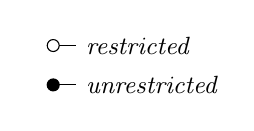
\begin{tikzpicture}[node distance=0.5cm]
  \node (p)  {};
  \node (p') [right of=p, anchor=west]  {\small\em restricted};
  \node (q)  [below of=p] {};
  \node (q') [right of=q, anchor=west] {\small\em unrestricted};

  \draw (p) edge [o-] (p')
        (q) edge [*-] (q')
  ;
\end{tikzpicture}
 \caption{Non-\converging typed topology in a hierarchical
  master-worker setting}
\label{fig:examplearch}
\end{figure}

Proposition \ref{p:one-bound} allows for further
applications, since it does not assume that the \qcp is finite: we can
combine locally decidable models for
multi-threaded programs (with or without local data), as
well as local event-based programs together with eager (or mutex)
communication architectures; natural candidates for local
models would be Petri Nets, well-structured transition systems~\cite{finkel-a-2001-63-a}, or
multi-set pushdown systems~\cite{sen-k-2006-300-a}.




\medskip \noindent{\it Summary.\ } We discussed
in detail the class of eager \rqcp (as well as mutex \qcp)
which both generalize the current lineup of decidable models
for asynchronously communicating pushdown systems. Further,
we presented an optimal decision procedure for eager
\rqcp over non-\converging architectures in \dexptime,
as well as  a direct and simpler construction
for bounded phase reachability for \rqcp.

\medskip \noindent{\it Outlook.\ } This paper dealt with the most basic form of verification, namely control-state
reachability. More general reachability questions
(w.r.t.~configurations) may be interesting to consider.
Further decision problems for \qcp, like boundedness or liveness, will
be investigated in future work.



 

\bibliographystyle{abbrv}

\bibliography{bibliography}
\end{document}
